\subsection{Desain Kontroler Robot}
\label{subsec:controllerdesign}

\begin{figure} [ht]
  \centering
  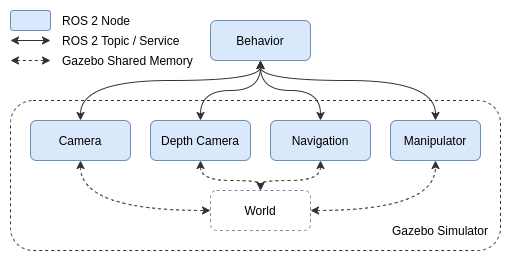
\includegraphics[width=0.45\textwidth]{images/simulation-controller.png}
  \caption{Diagram sistem kontroler robot di simulasi.}
  \label{fig:simulationcontroller}
\end{figure}

Kontroler robot yang digunakan untuk simulasi ini akan dikembangkan menggunakan ROS 2.
Kontroler tersebut akan dipisah menjadi beberapa bagian dalam bentuk \emph{ROS 2 node} seperti yang terlihat pada Gambar \ref{fig:simulationcontroller}.
Setiap \emph{node} yang ada akan terhubung satu sama lain menggunakan sistem komunikasi antar proses ROS 2 yang berupa \emph{topics} dan \emph{services}.

Bagian utama dari kontroler robot tersebut adalah \emph{node behavior} yang berisi program yang mengatur segala tindakan robot berdasarkan data yang didapat dari sensor yang ada di simulasi.
Kemudian \emph{node behavior} tersebut akan terhubung dengan empat \emph{node} lain yang merepresentasikan sensor dan aktuator yang ada pada robot.
Keempat \emph{node} tersebut akan terpasang di dalam cakupan simulator Gazebo sebagai \emph{Gazebo plugins},
  sehingga mampu digunakan untuk mengakses dan memanipulasi data yang ada di simulasi menggunakan sistem \emph{shared memory} pada Gazebo \citep{gazeboplugins}.

\begin{figure} [ht] \centering
  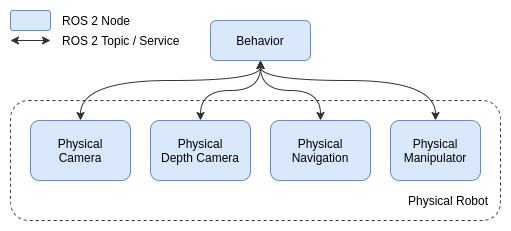
\includegraphics[width=0.45\textwidth]{images/real-robot-controller.png}
  \caption{Diagram sistem kontroler robot untuk robot fisik.}
  \label{fig:realrobotcontroller}
\end{figure}

Sistem ini dirancang secara terpisah agar \emph{node behavior} yang diujikan di lingkungan simulasi bisa langsung bekerja pada robot fisik.
Seperti yang terlihat pada Gambar \ref{fig:realrobotcontroller},
  transfer kontroler ke robot fisik dapat dilakukan dengan mengubah keseluruhan cakupan yang ada di simulator Gazebo,
  yang berupa empat \emph{node} yang telah disebutkan sebelumnya,
  menjadi \emph{node} yang memproses sensor dan aktuator yang ada pada robot fisik.
Dengan ini pengujian yang dilakukan di simulasi bisa langsung diterapkan ketika diujikan pada robot fisik karena tidak perlunya pembuatan ulang kontroler yang menyesuaikan sistem yang ada pada robot.
